\documentclass{report}
\usepackage[margin=1in, paperwidth=8.5in, paperheight=11in]{geometry}
%Math packages%
\usepackage{amsmath}
\usepackage{amsthm}
%Spacing%
\usepackage{setspace}
\onehalfspacing
%Lecture number%
\newcommand{\lectureNum}{9}
%Variables - Date and Course%
\newcommand{\curDate}{January 23, 2017}
\newcommand{\course}{MATH 239}
\newcommand{\instructor}{Luke Postle}
%Defining the example tag%
%\theoremstyle{definition}%
\newtheorem{ex}{Example}[section]
%Setting counter given the lecture number%
\setcounter{chapter}{\lectureNum{}}
%Package for drawing graphs%
\usepackage{tikz}
\usepackage{verbatim}
\usetikzlibrary{arrows}

\begin{document}
%Note title%
\begin{center}
\begin{Large}
\textsc{\course{} | Lecture \lectureNum{}}
\end{Large}
\end{center} 
\noindent \textit{Bartosz Antczak} \hfill
\textit{Instructor: \instructor{}} \hfill
\textit{\curDate{}}
\rule{\textwidth}{0.4pt}

% Actual Notes%
\subsubsection{Review of last lecture}
A subgraph $H$ of graph $G$ is \textbf{spanning} if $V(H) = V(G)$. A \textbf{spanning tree} $T$ of graph $G$ is a subgraph of $G$ that is a tree and is spanning. We also covered a \textit{theorem:}
\begin{center}
\textit{A graph $G$ is connected if and only if $G$ has a spanning tree}
\end{center}
The proof of this theorem went by removing edges from cycles. In particular, we chose a connected spanning subgraph $H$ with fewest edges and showed $H$ was a tree. We're going to look at an alternative proof in the ``right" ($\implies$) direction of our theorem: \textit{If G is connected, then G has a spanning tree}.
\subsubsection{Alternate Proof}
Let $H$ be a subgraph of $G$ that is a tree, and subject to that condition, $\vert V(H)\vert$ is maximized. Note that $H$ exists since any vertex of $G$ is such an $H$. I claim that $H$ is spanning. \\
Let's prove this with contradiction: suppose that $V(H) \neq V(G)$. Thus $V(H)$ is a proper subset of $V(G)$. Yet $V(H)$ is non-empty as $H$ has at least one vertex. Thus since $G$ is connected, the cut induced by $V(H)$ is non-empty. Now let $e$ be an edge in that cut. Let $H^\prime = H + e$. But now $H^\prime$ is a tree because it cannot contain a cycle with just vertices in $H$ and yet contain a cycle through its new vertex since it's a leaf (and clearly still connected). Yet $\vert V(H^\prime) \vert > \vert V(H) \vert$, which contradicts the minimality of $H$, thus proving that $H$ is spanning.\\
Indeed, this proof is algorithmic (which means that it can be converted to an algorithm), such that by `growing a tree', we either find a spanning tree $H$ which verifies that $G$ is \underline{connected}, or we find a subset $X = \vert V(H) \vert$ such that $\delta(X)$ is empty which verifies that $G$ is \underline{disconnected}.
\section{Eulerian Circuits}
\subsubsection{History}
Back in the day (1700's), there was an old problem of whether a citizen of Konigsberg (now in current-day Kaliningrad) could traverse all the bridges of Konigsberg without using a bridge twice and returning to their starting location.\\
The mathematician given the task of solving this problem was Euler! (What \textit{can't} this man do?) After some analyzation, Euler realized that this was a graph theory problem as follows:
\begin{center}
\textit{Does there exist a walk $W$ such that $W$ contains all the edges of $G$ but every edge at most once, and such a walk $W$ is closed (i.e., same start and end)}
\end{center}
\newpage
\begin{ex}
Various graphs ($K_3, K_4, K_5$)
\end{ex}
%K_3%
\begin{center}
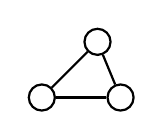
\begin{tikzpicture}[-,auto,node distance=1cm,
                    thick,main node/.style={circle,draw,font=\sffamily\small}]

  \node[main node] (1) {};
  \node[main node] (2) [above right of=1] {};
  \node[main node] (3) [right of=1] {};

  \path[every node/.style={font=\sffamily\small}]
    (1) edge node [left] {} (2)
    	edge (3)
    (2) edge node [left] {} (3);
\end{tikzpicture}
$\qquad$
%K_4%
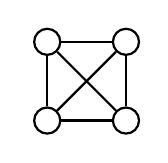
\begin{tikzpicture}[-,auto,node distance=1cm,
                    thick,main node/.style={circle,draw,font=\sffamily\small}]

  \node[main node] (1) {};
  \node[main node] (2) [above of=1] {};
  \node[main node] (3) [right of=2] {};
  \node[main node] (4) [right of=1] {};

  \path[every node/.style={font=\sffamily\small}]
    (1) edge node [left] {} (2)
    	edge (3)
    	edge (4)
    (3) edge node [left] {} (4)
    	edge (2)
    (2) edge (4);
\end{tikzpicture}
$\qquad$
%K_5
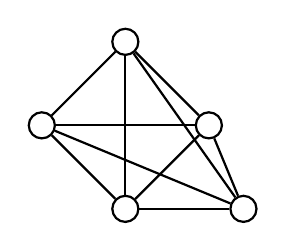
\begin{tikzpicture}[-,auto,node distance=1.5cm,
                    thick,main node/.style={circle,draw,font=\sffamily\small}]

  \node[main node] (1) {};
  \node[main node] (2) [above right of=1] {};
  \node[main node] (3) [below right of=2] {};
  \node[main node] (4) [below right of=1] {};
  \node[main node] (5) [right of=4] {};

  \path[every node/.style={font=\sffamily\small}]
    (1) edge node [left] {} (2)
    	edge (3)
    	edge (4)
    (3) edge node [left] {} (4)
    	edge (2)
    (2) edge (4)
    (5) edge (1)
   		edge (2)
	    edge (3)
    	edge (4)
	    edge (5);	    
\end{tikzpicture}
\end{center}
Observe that only $K_3$ and $K_5$ satisfy this property that Euler was looking for. From this, we arrive at an observation: only graphs of odd degree are Eulerian circuits.
\subsection{Definition}
An \textbf{Eulerian Circuit} of a graph $G$ is a closed walk that uses every edge exactly once.\\
Naturally one would ask, \textit{when does $G$ have an Eulerian circuit}?
\subsubsection{Proposition 1}
\begin{center}
\textit{If $G$ has a vertex $v$ of \underline{odd degree}, then $G$ does not have an Eulerian circuit.}
\end{center}
\textbf{Proof of Proposition 1:} if a vertex of an odd degree did have an Eulerian circuit, then we could pair the edges incident to $v$ by how they appear consecutively in the walk. But then $v$ has even degree, which is a contradiction. \\
From this, we ask another question: \textit{if $G$ has all even degrees does it have an Eulerian circuit}? The answer is \textbf{no}. Consider the following graph as a counter-example:
\begin{center}
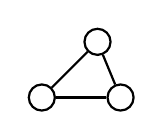
\begin{tikzpicture}[-,auto,node distance=1cm,
                    thick,main node/.style={circle,draw,font=\sffamily\small}]

  \node[main node] (1) {};
  \node[main node] (2) [above right of=1] {};
  \node[main node] (3) [right of=1] {};

  \path[every node/.style={font=\sffamily\small}]
    (1) edge node [left] {} (2)
    	edge (3)
    (2) edge node [left] {} (3);
\end{tikzpicture}
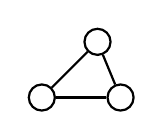
\begin{tikzpicture}[-,auto,node distance=1cm,
                    thick,main node/.style={circle,draw,font=\sffamily\small}]

  \node[main node] (1) {};
  \node[main node] (2) [above right of=1] {};
  \node[main node] (3) [right of=1] {};

  \path[every node/.style={font=\sffamily\small}]
    (1) edge node [left] {} (2)
    	edge (3)
    (2) edge node [left] {} (3);
\end{tikzpicture}
\end{center}
The graph has all vertices of even degree, yet it is not an Eulerian circuit because no such walk exists that uses all edges at most once. We'll outline this property in a proposition:
\subsubsection{Proposition 2}
\begin{center}
\textit{If a graph $G$ has edges in two different components, then $G$ does not have an Eulerian circuit.}
\end{center}
\textbf{Proof of Proposition 2:} if there was a circuit, then a walk $W$ would connect such edges, but since they're in different components, they can't be connected.\\
From these questions, Euler defined the following theorem:
\subsection{Theorem 1 (by Euler)}
\begin{center}
\textit{Graph $G$ has an Eulerian circuit if and only if all of the vertex's degrees are even and all edges are in the same component}
\end{center}
\textbf{Proof of Theorem:}
\begin{itemize}
\item Proof of $\implies$: \textit{G is an Eul. circuit then all degrees even and edges are conected}\\
We proved this in the previous two propositions.
\item Proof of $\impliedby$: \textit{if all edges connected and vertices even, then G is an Eul. circuit}\\
Before we prove this, let's define an easy lemma:
\subsubsection{Lemma 1}
\begin{center}
\textit{If G is a graph will all even degrees and $e$ is an edge of $G$, then there exists a closed walk using no edge more than once and containing $e$}
\end{center}
\textbf{Proof of Lemma 1:} Let $W$ be a walk using no edge more than once and containing $e$, and subject to that $\vert E(W) \vert$ is maximised. Note $W$ exists since $e$ is such a walk. I claim that $W$ is closed.
Let's prove this claim by contradiction. Suppose that $W$ is not closed. Then the first vertex of $W$ is not its last, so only an \underline{odd} number of edges incident with the last vertex $v$ are in $W$. Since $v$ has even degree, there exists an edge $f \not\in W$ and incident with $v$. But then, $W^\prime = W - f$ is a longer walk using no edge more than once and containing $e$, contradiction that $\vert E(W)\vert$ is maximized.\\\\
Now to the main proof. Let $W$ be a closed walk of $G$ using no edge more than once and subject to that, $\vert E(W) \vert$ is maximized. Note that $W$ exists since if there exists an edge $e$, then there exits a closed walk using no edge more than once and containing $e$ by the lemma. \\
If $G$ has no edges, then $G$ trivially has an Eulerian circuit, so we're done. Otherwise, I claim that $W$ use all the edges of $G$. To prove this, we'll use contradiction. Suppose that there exists an edge $e$ not in $W$ with at least one end in $W$  since all edges are in same component. By the lemma, applied to $G^\prime = G - E(W)$, there exists a closed walk containing $W^\prime$. But then if you insert $W^\prime$ into $W$, you get a larger closed walk, contradicting the maximality.
\end{itemize}
%END%
\end{document}